\documentclass[12pt,a4paper]{report}
\synctex=1
\usepackage[utf8]{inputenc}
\usepackage[margin=2cm, top=1.5cm, bottom=2cm]{geometry}

\usepackage{graphicx}
\usepackage{libertine}
\usepackage{amsmath}
\usepackage{amssymb}
\usepackage{listings}
\usepackage{pgfornament}
\usepackage{eso-pic}
\usepackage{textcomp}
\usepackage{courier}
\usepackage[hangul]{kotex}
\usepackage{rotating}
\usepackage{dirtree}

\title{
	\centering
	\pgfornament[width=12cm,color=teal]{84}\\
	\vspace{1cm}
	\fontsize{50}{50} \selectfont {File Browsesr\\inspired by MindMap}\\
		\pgfornament[width=12cm,color=teal]{88}\\
	\vfill}
\author{
	\LARGE
	\begin{tabular}{rl}
		\hline
		교과목명 : & 컴퓨터 알고리즘과 실습\\
		담당교수 : & 주 종화 교수님\\
		프로젝트명 : & File's Mind\\
		학번 : & 2016110056\\ 
		이름 : & 박승원\\
		날짜 : & \today\\
		\hline
	\end{tabular}\vspace{1cm}
	\\
\includegraphics[width=0.5\textwidth]{logo.jpg}
	}
\date{}


\linespread{1.3}

\begin{document}

\maketitle

%\includegrap

\newpage
\tableofcontents
\newpage
\chapter*{Summary}
\paragraph{Project name} File browser inspired by MindMap\\ 
\paragraph{Keyword} File Browser, Mindmap, Graph, Tree\\
\paragraph{1. Objective} Make a file browser that is intuitive, easy to search and show data in structured way\\
\paragraph{2. How} using C++ and Makefile project\\
\paragraph{3. Result} Very efficient and intuitive file browser is made. There is a possibility that it can be also used as an IDE.
\paragraph{4. Analysis} Graph structure was a good choice to implement Directory organization\\

\noindent
\chapter{Introduction}
\section{Project Objective}
Learning Computer Science, I received many documents and data. These data were to be referenced often
and stored well. But, it was very hard to remember where I put those files. Every time I wander directories
searching for the files, I felt weary. So, I needed a way to systemically store files and show it in a orderly form.
I reminded the Mindmap. Mindmap was somewhat a tree data structure. And directories are definately a
tree. So I thought I can make a mindmap-like file browser.
\section{Project Content}
I used graph sturcture to represent those files and directories. Because tree structure is a form of graph, I
reconfigured the graph header file I made in data structure class of last semester to fit my needs.
Basic idea is to show what I want to show(among directories and files) at the place where I want to show
them(in a big sketchbook).

\section{Project Progress}

\begin{tabular}{|c|c|}
	\hline
	세부 개발내용&주별 세부 추진 일정\\
	\hline
	자료수집 및 설계 계획 수립&$\sim$ 3/16\\
	요구사항 검토&3.17\\
	구조도 및 모듈 설계&4.18\\
	프로그램 설계&5.19\\
	프로그램 코딩&5.20$\sim$ 5.25\\
	성능확인 및 오류 수정&5.26\\
	최종 점검 및 개선 사항 보완&5.27\\
	\hline
\end{tabular}
\chapter{Program Structure and Making}
\section{Usage}
Program should be executed in command line in linux.
First argument is the directory name that I want to show.
All the subdirectories will be shown in the program.

By default, directories are shown in an ellipse and files are hidden.
Right clicking on the directory or files will bring a popup menu.
\begin{itemize}
	\item shape : set rim, arrow style and alpha, change file name
	\item color : set color of text, rim, arrow
	\item open : open file or directory
	\item resize : set rim size
	\item expose : this menu is shown only in directories. Clicking on this will bring up a file chooser. The chosen file will be shown on the screen. In this way you can select which files to show and which files not to show.
	\item cancel : cancel
\end{itemize}
If you drag a node to a new position, program will remember the position and save it when you exit.
If you drag a node onto other directory, it will move the file to the directory.

By combining these simple procedures, you can make a mindmap-like structure.

\section{Figure of program structure}
Picture down below shows sources of this project by using this program itself.
mindmap.h and special.h(template specialization of tgraph.h) is the header file containing main classes.


It shows that even programming project can be explained by grouping files and commenting some lines.

\begin{sidewaysfigure}
	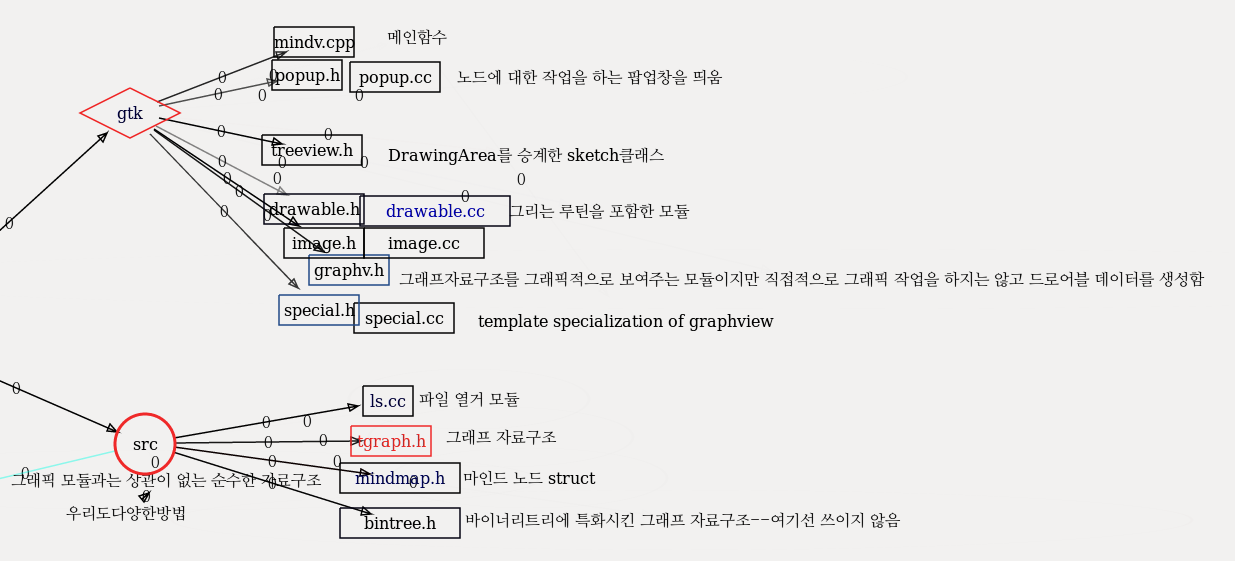
\includegraphics[width=\textwidth]{3.png}
	\caption{Source file structure shown with this program}
	\label{tree}
\end{sidewaysfigure}


\begin{sidewaysfigure}
	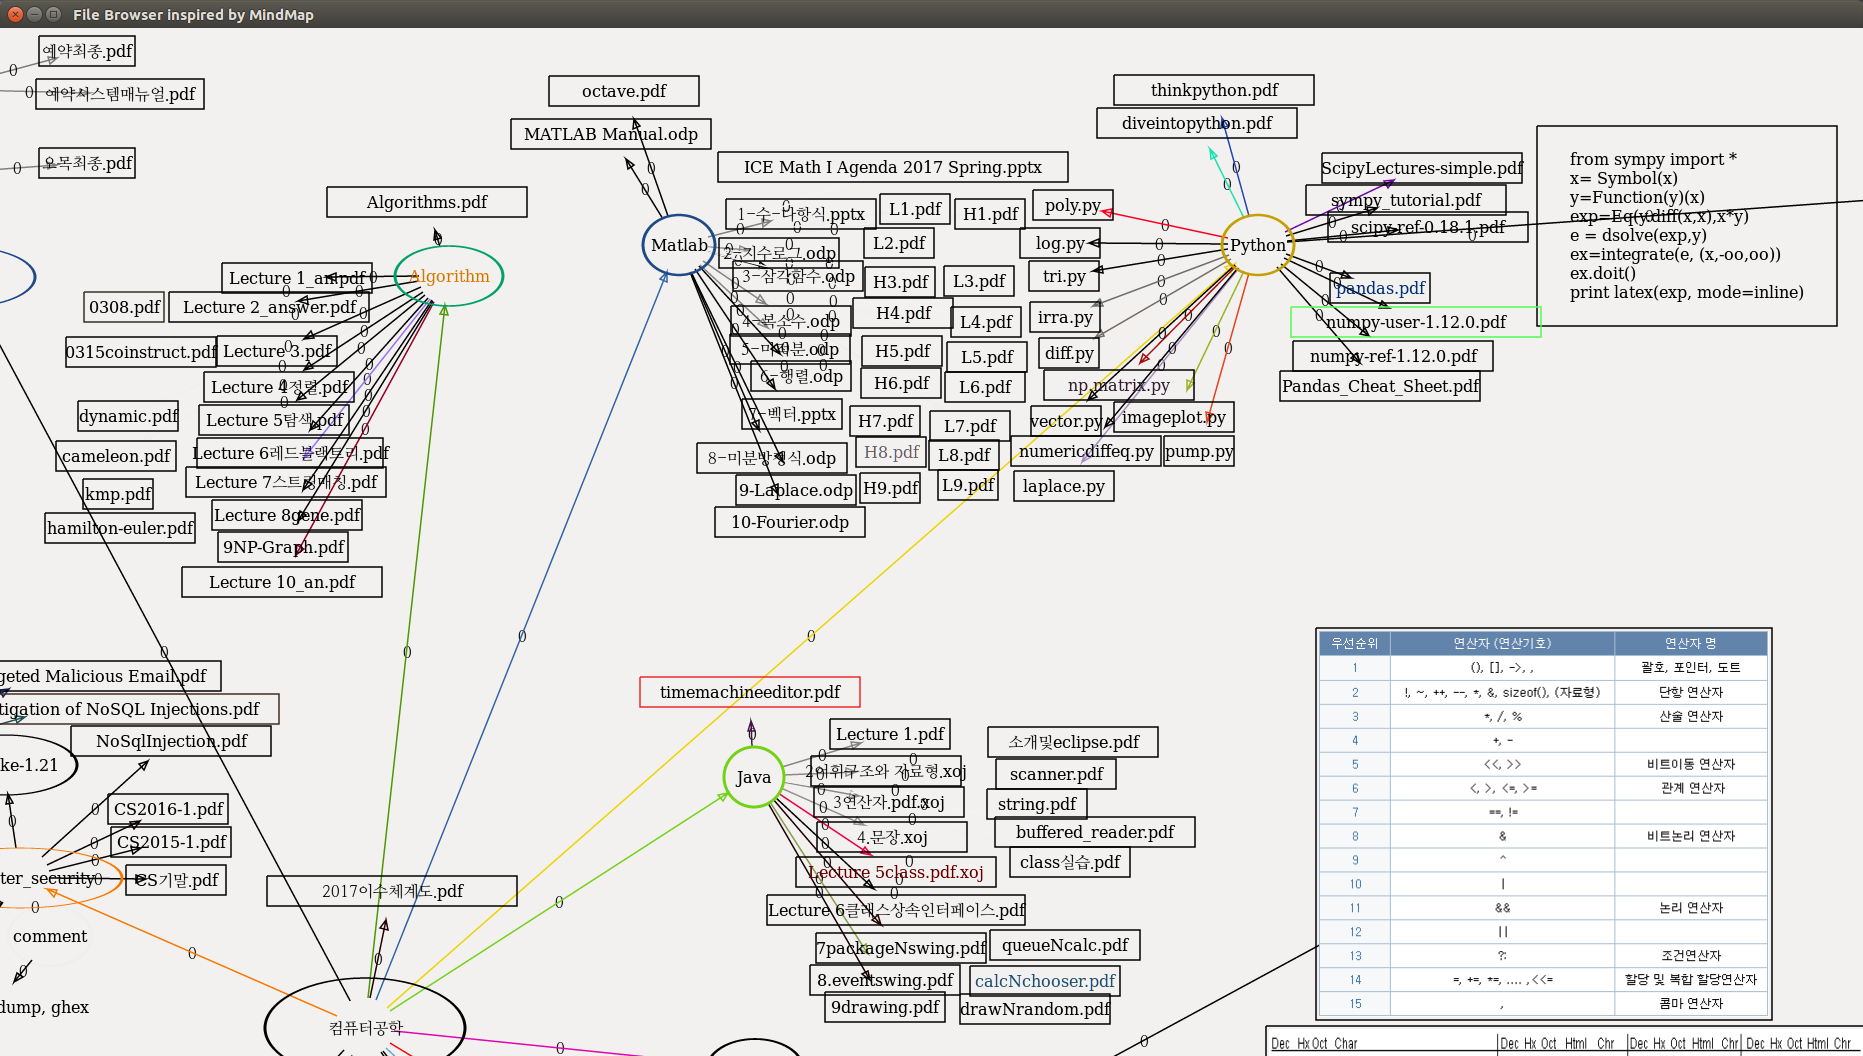
\includegraphics[width=\textwidth]{1.png}
	\caption{Execution screen of File Browser}
	\label{data}
\end{sidewaysfigure}

\newpage
\section{Detailed explanation of Program}

\subsection{tgraph.h}

\paragraph{Edge class} template class that represent graph edge 
\paragraph{Vertex class} template class that represent graph vertex
\paragraph{Graph} template class that represent graph structure and manipulating it

\subsection{special.h}
Reconfigured GraphView class to fit Mindmap tree.

\subsection{mindmap.h}
Graph class will deal with this mindmap class as a data.
\subsection{graphv.h}
Data structure to show Graph in a mindmap like format.

\subsection{drawable.h}
Drawing routine with gtkmm library.
\chapter{Result and Discussion}

\section{Result and Performance}

I used python script to open files. Python webbrowser module automatically detect file extension and call a proper program.

Program was very fast. But there could be some bugs especially in dealing with moving files and reconsructing mindmap.

Saving current state was done automatically in destructor. But, I had to restart again to make change applied. This can be improved by a little coding.

\section{Discussion}
I already began this project from the beginning of this semester. I
am now using it and benefitting from it. Now it is so easy to find and open a file I want to see. It is just one click
away.

When I code a program, this program will also help me remember what file is about what procedure.
And I can open the file in an editor with a click.

When I store files, I can selectively emphasize certain files and order files in a structured way. 
Commenting is also achieved by adding a directory of file names which is a comment string.
This is somewhat walk-around, but this made program structure very simple.

Showing files in a Mindmap like style is also possible.
This program is tightly connected with file system, so that not just showing text and icons but also using any kind of file such as video or pdf files can be very useful.

People are just tied to one concept of File browser. 
It is showing folders and sorting files in a rectangle.
File browser is the basic of basic in computer system.
If we make it more intuitive and more efficient and rememberable, we will benefit from it very much.
\section{Etc}
If this program is polished well enough, it can alse be used as an IDE.
This is just a possibility but, I think, using mindmap like IDE is the future.
IDE is just a file browser from my point of view.
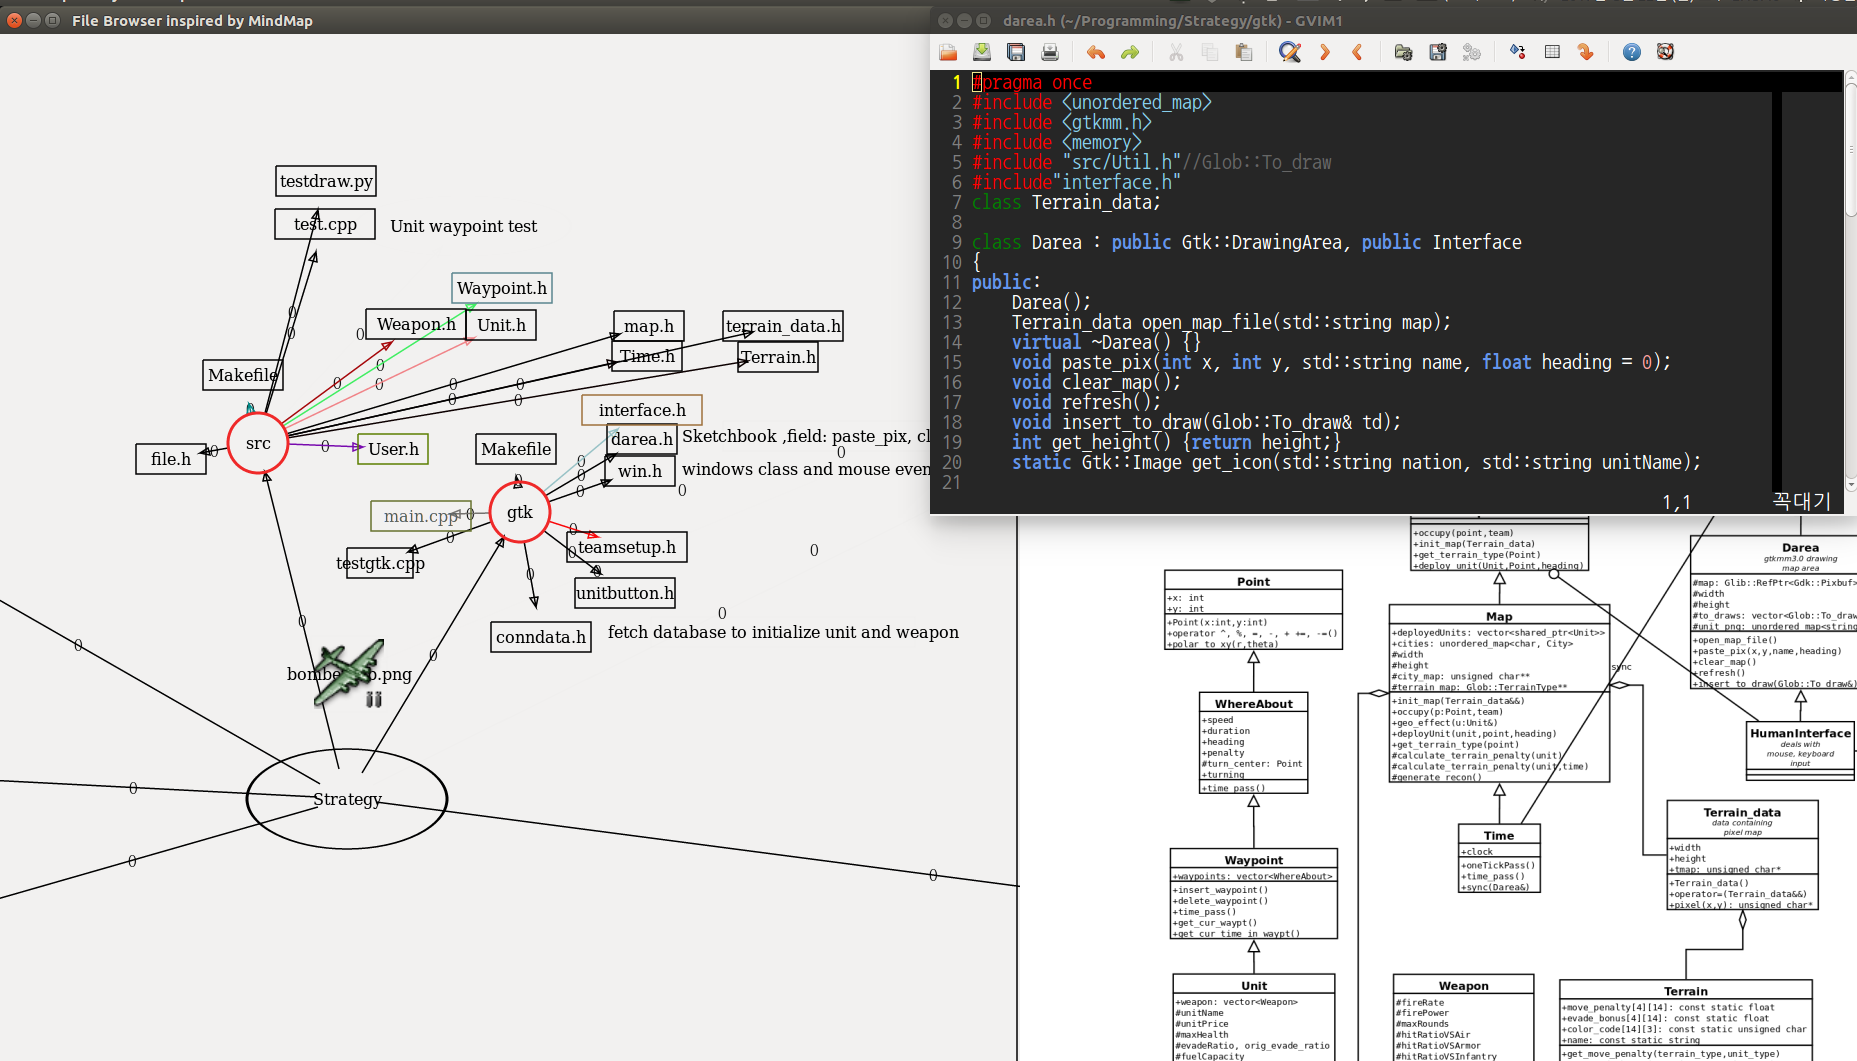
\includegraphics[width=\textwidth]{2.png}
\chapter{Attachment}
Source code attached separately
\end{document}
